\documentclass[12pt,a4paper]{article}

\usepackage[margin=1in,top=1.25in,bottom=1.25in]{geometry}
\usepackage[T1]{fontenc}
\usepackage[utf8]{inputenc}
\usepackage{lmodern}
\usepackage{microtype}
\usepackage{setspace}
\usepackage{amsmath,amssymb}
\usepackage{booktabs}
\usepackage{longtable}
\usepackage{graphicx}
\usepackage{float}
\usepackage[hidelinks,breaklinks]{hyperref}
\usepackage[authoryear,round,sort]{natbib}

\setlength{\tabcolsep}{3.5pt}   % tables are wide; keep them inside the text block
\setlength{\parindent}{1.5em}
\setlength{\parskip}{0.3em}

%% \input before \bottomrule breaks booktabs (Misplaced \noalign); the primitive does not.
\makeatletter\newcommand{\tabinput}[1]{\@@input #1.tex }\makeatother

% Generated by code/12_make_numbers.py. Do not edit by hand.
\newcommand{\dataDate}{5 October 2026}
\newcommand{\dataMonth}{October 2026}
\newcommand{\versionId}{2026-10-05}
\newcommand{\firstOpen}{June 2021}
\newcommand{\nMarkets}{50,157}
\newcommand{\nSeries}{652}
\newcommand{\nEvents}{4,588}
\newcommand{\reMarkets}{1,669}
\newcommand{\reSeries}{65}
\newcommand{\reVolM}{3.4}
\newcommand{\totalVolM}{1,206}
\newcommand{\reVolShare}{0.3}
\newcommand{\priceVolM}{0.35}
\newcommand{\priceSeries}{28}
\newcommand{\rentZeroShare}{56}
\newcommand{\reMaxHorizon}{537}
\newcommand{\priceMaxHorizon}{412}
\newcommand{\reMaxHorizonMonths}{18}
\newcommand{\reMedianVol}{284}
\newcommand{\otherMedianVol}{998}
\newcommand{\topTenShare}{81}
\newcommand{\fedVolM}{618}
\newcommand{\cmeRatio}{1,700}
\newcommand{\allVolBn}{177}
\newcommand{\sportsVolBn}{130}
\newcommand{\sportsShare}{73}
\newcommand{\sportsToRe}{38,000}
\newcommand{\reShareAll}{0.002}
\newcommand{\sportsSeriesBigger}{640}
\newcommand{\adjSeries}{3}
\newcommand{\adjMarkets}{32}
\newcommand{\adjVol}{23,000}
\newcommand{\adjFirst}{June 2026}
\newcommand{\adjVolShareOfRe}{0.7}
\newcommand{\regEvents}{4,036}
\newcommand{\regSeries}{432}
\newcommand{\regReEvents}{274}
\newcommand{\regPriceEvents}{28}
\newcommand{\uncondGap}{81}
\newcommand{\condGap}{71}
\newcommand{\strikeElasticity}{$-$0.6}
\newcommand{\priceMedianStrikes}{7}
\newcommand{\reEventsManyStrikes}{23}
\newcommand{\quoteMarkets}{5,999}
\newcommand{\quoteReMarkets}{1,242}
\newcommand{\spreadRe}{6}
\newcommand{\spreadOther}{6}
\newcommand{\spreadRoundTrip}{12}
\newcommand{\spreadComparison}{6 cents in both groups}
\newcommand{\twoSidedRe}{70}
\newcommand{\twoSidedOther}{61}
\newcommand{\twoSidedGap}{12}
\newcommand{\priceDaysTraded}{25}
\newcommand{\rentDaysTraded}{22}
\newcommand{\otherDaysTraded}{39}
\newcommand{\brierRe}{0.120}
\newcommand{\brierOther}{0.091}
\newcommand{\brierDiff}{0.009}
\newcommand{\calSlope}{1.04}
\newcommand{\priceForecastN}{136}
\newcommand{\spreadStrikeCoef}{$-$2.4}
\newcommand{\spreadBinMin}{4}
\newcommand{\spreadBinMax}{6}
\newcommand{\spreadReOneStrike}{3}
\newcommand{\spreadReManyStrikes}{8}
\newcommand{\cookSalesM}{2.4}
\newcommand{\cookSalesDate}{4 October 2026}
\newcommand{\nycSalesDate}{4 October 2026}
\newcommand{\caseShillerDate}{5 October 2026}
\newcommand{\pairs}{466,402}
\newcommand{\pairProperties}{308,963}
\newcommand{\hedgeUnderTwo}{0.9}
\newcommand{\hedgeTwoThree}{17}
\newcommand{\hedgeThreeFive}{37}
\newcommand{\hedgeFiveTen}{44}
\newcommand{\hedgeTenPlus}{31}
\newcommand{\binaryThreeFive}{31}
\newcommand{\binaryTenPlus}{15}
\newcommand{\earlyThreeFive}{44}
\newcommand{\earlyFiveTen}{36}
\newcommand{\lateThreeFive}{4}
\newcommand{\lateFiveTen}{7}
\newcommand{\sdIndexEarly}{0.25}
\newcommand{\sdIndexLate}{0.11}
\newcommand{\nycMaxR}{0.2}
\newcommand{\polyEvents}{64}
\newcommand{\polyPriceVolM}{1.56}
\newcommand{\polyLaunch}{January 2026}
\newcommand{\polyMaxHorizon}{102}
\newcommand{\polyBracketsMin}{5}
\newcommand{\polyBracketsMax}{9}
\newcommand{\polyMetros}{9}
\newcommand{\polyJanMedian}{21,000}
\newcommand{\polyMarJunMedian}{6,000}
\newcommand{\polyJulyMedian}{100,000}
\newcommand{\polyMortgageEvents}{7}
\newcommand{\polyOtherEvents}{2}
\newcommand{\polyTx}{37,057}
\newcommand{\polyWallets}{3,443}
\newcommand{\polyTakerUsd}{848,000}
\newcommand{\polyTakerUsdM}{0.85}
\newcommand{\walletMedianUsd}{20}
\newcommand{\walletUnderHundred}{75}
\newcommand{\walletOneMonth}{90}
\newcommand{\bigWallets}{19}
\newcommand{\topTenWalletShare}{33}
\newcommand{\mmWallets}{990}
\newcommand{\mmShare}{34}
\newcommand{\holdWallets}{1,291}
\newcommand{\holdShare}{39}
\newcommand{\bigHold}{9}
\newcommand{\bigRound}{5}
\newcommand{\bigMM}{5}
\newcommand{\bigRestHold}{0}
\newcommand{\bigMedianMarkets}{4,900}
\newcommand{\bigRewarded}{12}
\newcommand{\bigRewardedLarge}{3}
\newcommand{\topProfiled}{25}
\newcommand{\housingOnly}{2}
\newcommand{\topWalletShare}{8}
\newcommand{\topWalletUsd}{109,000}
\newcommand{\hedgerCandidates}{95}
\newcommand{\hedgerOneArea}{3}
\newcommand{\hedgerLike}{1}
\newcommand{\hedgerLikeUsd}{1,200}
\newcommand{\maxNetPosition}{32,000}
\newcommand{\depthDate}{5 October 2026}
\newcommand{\depthKalshiEvents}{15}
\newcommand{\depthKalshiMedian}{3,300}
\newcommand{\depthKalshiMax}{11,700}
\newcommand{\depthKalshiBookMedian}{6,000}
\newcommand{\depthPolyEvents}{10}
\newcommand{\depthPolyMedian}{2,600}
\newcommand{\depthPolyMax}{7,500}
\newcommand{\depthPolyBookMedian}{12,100}
\newcommand{\depthMaxShare}{23}
\newcommand{\depthMedianShare}{6}
\newcommand{\fillHundred}{99}
\newcommand{\fillNearHundred}{83}
\newcommand{\moveHundred}{0}
\newcommand{\fillThousand}{52}
\newcommand{\fillNearThousand}{13}
\newcommand{\moveThousand}{39}
\newcommand{\fillLadder}{7}
\newcommand{\fillNearLadder}{1}
\newcommand{\moveLadder}{66}
\newcommand{\fillFull}{0}
\newcommand{\fillNearFull}{0}
   % every number in the prose; generated by code/12_make_numbers.py

\newif\ifanon
\anonfalse   % <── change to \anontrue for blind submission

\begin{document}
\begin{center}
  \vspace*{0.5em}
  {\large\bfseries\singlespacing Real Estate Derivatives at Last? An Exploration of Prediction Markets}\\[1.5em]
  \ifanon
    {\small\textit{Submitted for blind review}}\\[0.3em]
  \else
    {\normalsize
      Thies Lindenthal\\[0.4em]
      Department of Land Economy, University of Cambridge\\[0.2em]
      \texttt{htl24@cam.ac.uk}}\\[1.2em]
    {\small\textit{Draft with data to \dataDate{}. Preliminary results.}}\\[0.3em]
  \fi
\end{center}

\noindent\rule{\textwidth}{0.4pt}

\begin{abstract}
\noindent\small Exchanges have listed derivatives on property prices since 1991 and none has become liquid. Event contracts on prediction markets are the latest attempt: binary claims on house price indices, rents and mortgage rates, sold in one-dollar units to retail traders. This paper asks whether that architecture removes the obstacles that stopped earlier property derivatives. It does not. Between \firstOpen{} and \dataMonth{} Kalshi listed \reMarkets{} real estate contracts in \reSeries{} series. Together they traded \reVolM{} million contracts, \reVolShare{} per cent of the volume in the exchange's economics category, and a real estate event trades about \condGap{} per cent less than a comparable economics event. House price contracts on Polymarket have traded \polyPriceVolM{} million contracts since \polyLaunch{}, for which buyers paid \polyTakerUsdM{} million dollars; the median account traded \walletMedianUsd{} dollars, \walletOneMonth{} per cent of accounts never returned, and the large accounts are generalist bettors and liquidity providers. The contracts are nonetheless quoted as tightly and priced as accurately as other economics contracts. They forecast; they do not transfer risk. Nor could they at the horizons listed. In \pairs{} repeat sales in Cook County, Illinois, a hedge on the Case-Shiller Chicago index removes \hedgeUnderTwo{} per cent of house-level price variance or less for holdings below two years and \hedgeFiveTen{} per cent at five to ten years, and that larger share comes from the 2000s boom and bust alone. A ladder of seven binary contracts hedges as well as a future. No real estate contract on Kalshi runs longer than \reMaxHorizonMonths{} months. The paper is built to be re-run: every number in it is recomputed from the exchanges' public data when the pipeline runs.
\end{abstract}

\noindent\rule{\textwidth}{0.4pt}

\newpage
\onehalfspacing

\section{Introduction}

Housing is the largest asset most households own, and they cannot hedge it. Real estate as a whole is the largest asset class without a liquid derivatives market \citep{geltner2007pricing,fabozzi2020thirty}: US households and nonprofits alone own about 30 trillion dollars of it, close to the value of the US equity market, and neither a homebuyer nor an investor in mortgage-backed securities has a straightforward way to hedge against a fall in its price \citep{fabozzi2020thirty}. \citet{case1993index} proposed cash-settled futures and options on house price indices to close that gap, and \citet{shiller1999home} followed with insurance policies in which an insurer retails short index positions to homeowners. The case for demand has held up reasonably well since then: \citet{englund2002hedging} estimate large gains from instruments that would let households hedge their housing investment, largest for poorer owners, although \citet{sinai2005owner} point out that owning a home is itself a hedge against rent risk and that for most households this risk outweighs the risk in house prices. Supply has been tried repeatedly and has failed each time. \citet{shiller2008derivatives} recounts the attempts up to 2007 and \citet{fabozzi2020thirty} take stock thirty years on, naming four obstacles: settlement indices that fit the contracts badly, a fear of negligible liquidity in a market where nearly everyone wants the same side, the lack of an accepted pricing model, and regulation. For liquidity they look to pension funds, insurers and hedge funds, with general investors coming last, as people who might be enticed once a market is established.

Prediction markets now list contracts on the same underlying statistics. A contract pays one dollar if, say, the FHFA house price index rises by more than a stated amount, and nothing otherwise, which is the all-or-nothing contract that \citet{manski2006interpreting} describes as the instrument traded in prediction markets. It differs from a futures contract in two ways that matter here. The payoff is a claim on a state and not a linear exposure, so that a ladder of strikes traces out a whole distribution, and the buyer is someone with a phone and a brokerage app, not an institution with a clearing account \citep{diercks2026kalshi}. The hope is that speculators who enjoy taking a view on house prices will supply the liquidity that hedgers never managed to supply to each other. That speculators make a market deep enough for hedgers to use is an old observation about futures markets \citep{pagano1989trading}, and who trades a new contract, hedgers or speculators, is known to affect whether it survives \citep{bekkerman2017revisiting}.

This paper tests that hope on Kalshi,\footnote{\url{https://kalshi.com}. Market data come from the exchange's public API at \url{https://api.elections.kalshi.com/trade-api/v2}.} which \citet{diercks2026kalshi} describe as the largest federally regulated prediction market, with Polymarket\footnote{\url{https://polymarket.com}. Event and trade data come from \url{https://gamma-api.polymarket.com} and \url{https://data-api.polymarket.com}.} as a second case. It looks at whether real estate event contracts trade at all, how they compare with contracts on other economic statistics listed on the same exchange, and whether listing many strikes per event, the feature that makes them informative, costs them liquidity.

They barely trade. All house price contracts listed on Kalshi since \firstOpen{} traded \priceVolM{} million one-dollar contracts between them (Table~\ref{tab:inventory}), whereas the CME housing futures that are usually described as a failure traded 612 million dollars of notional in their first eighteen months \citep{shiller2008derivatives}, about \cmeRatio{} times as much. A real estate event also trades roughly \condGap{} per cent less than an economics event with the same listing period and number of strikes on the same exchange (Table~\ref{tab:regression}), while the evidence that additional strikes thin out trading is suggestive at best. Polymarket launched house price contracts in \polyLaunch{} and has reached the same order of magnitude as Kalshi, and because its trade records are public they also show who takes part, which is mostly accounts that trade a few dollars once and do not return (Table~\ref{tab:wallets}).

I do not think this is a slow start that time will fix. The contracts are perfectly good forecasts: they are quoted on most days, at the same spreads as other economics contracts, and their prices are as well calibrated (Table~\ref{tab:quotes}), which is what the literature on prediction markets would lead one to expect \citep{wolfers2004prediction,diercks2026kalshi}. What they cannot do is hedge. Repeat sales in Cook County show that an index-settled contract removes almost none of an owner's price risk at holding periods under two years (Table~\ref{tab:hedging}), which is in line with the large idiosyncratic component of house price risk that \citet{giacoletti2021idiosyncratic} documents, and neither exchange lists anything longer. A ladder of binary contracts would hedge as well as a future if it ran for five years and somebody traded it, so the obstacle is the horizon and the basis, and neither a new payoff nor a better app does anything about those.

The architecture is also less new than it looks. \citet{shiller2008derivatives} describes HedgeStreet, which in 2004 offered consumers ten-dollar bets on the direction of home prices through a dedicated website and closed for lack of trade, and \citet{fabozzi2020thirty} add that these contracts were binary, paying off if a house price index for one of six cities fell within a stated range over the next three months. The same authors report that UK spread-betting firms had offered bets on house prices from 2001, which were seen as gambling and not as hedging instruments and traded sparsely. \citet{gurkaynak2006macroeconomic} study a market that Goldman Sachs and Deutsche Bank opened in 2002, in which ten to twenty digital options at different strikes were auctioned on each macroeconomic data release, so that a full distribution of outcomes could be read from the prices; they find those prices remarkably well calibrated. Contracts on housing statistics other than prices are older still: \citet{carlton1984futures} mentions that the Coffee, Sugar and Cocoa Exchange had proposed futures on the number of housing starts in the early 1980s. Retail binary bets on house prices and tradable distributions over economic statistics were thus both tried twenty years ago, and the difference now lies in how many people trade event contracts.

\section{Thirty years of property derivatives}

The record is set out by \citet{shiller2008derivatives} and \citet{fabozzi2020thirty}, and the facts in this section come from those two accounts unless another source is given. Case, Shiller and Weiss took the idea of a house price future to the Chicago Board of Trade in 1990, but a survey in 1993 showed plenty of interest in protection against falling prices and little in selling it, and the exchange decided not to launch. The London Futures and Options Exchange did launch futures on residential and commercial property in May 1991, with the housing contract settling on the Nationwide index; there was little trade, traders padded the volume with wash trades, and the contracts were terminated in October of the same year. Goldman Sachs listed covered warrants on UK house price indices in 2003, and by 2004 the open interest was roughly what would hedge a hundred houses. HedgeStreet followed in 2004 with the retail binary contracts described above, prompting \citet{shiller2008derivatives} to remark that it has seemed hard to get hedging markets started for real estate.

The CME launched futures and options on the S\&P/Case-Shiller indices for ten cities and a composite in May 2006. According to \citet{shiller2008derivatives}, notional value traded reached 612 million dollars by November 2007, while open interest in the futures peaked at 109 million dollars in February 2007 and had fallen to 49 million by November; maturities of up to five years were added in September 2007. \citet{fabozzi2020thirty} report that the market peaked around the subprime crisis and survives only in diminished form. The contract was not useless on paper, since \citet{bertus2008hedging} calculate that CME futures would have removed more than 88 per cent of house price risk for a holder of a mix of new and existing homes in Las Vegas over 1994--2006, a backtest on index data that predates the contract. In commercial property the picture was somewhat better in the UK, where swaps on the IPD index traded more than three billion pounds of notional in the first quarter of 2007, than in the US, where no single index commanded the same acceptance \citep{geltner2007pricing,fabozzi2020thirty}.

The literature offers several explanations for why these markets stay thin, and an event contract touches only some of them. The first is the settlement index: \citet{clapham2006revisiting} show that repeat-sales indices are revised substantially and systematically downward as new sales arrive, which is awkward for a contract that must settle on one published number, and \citet{geltner2007pricing} find that a lack of confidence in how index derivatives should be priced was among the two most important barriers named by US investment managers in 2006. The second is basis risk, because a homeowner owns one house and not the index. \citet{dejong2008hedging} build both into a portfolio model and find that access to city-level housing futures improves a homeowner's welfare only slightly, since the idiosyncratic risk of the individual house remains, and \citet{giacoletti2021idiosyncratic} measures that risk and shows that it accounts for a large fraction of house price variance, a fraction that falls as the holding period lengthens. \citet{eichholtz2021total} extend the decomposition from prices to total returns, using repeated observations of both prices and rents for individual houses in Amsterdam. They find that in the short term nearly all total return risk is idiosyncratic and comes from capital gains, that the idiosyncratic part still makes up about half of gross total return risk at holding periods of fifteen years and more, and that over long horizons a growing share of it stems from rental yields, which are persistent at the level of the individual property. For an investor who holds a house for its rent as well as its price, a contract on a price index therefore leaves a second idiosyncratic component untouched, and one that does not fade with time. The third is the missing counterparty, since almost every household and lender is naturally long, which is the one-sidedness that the Chicago survey of 1993 found and that \citet{fabozzi2020thirty} still list among the main obstacles. \citet{shiller2008derivatives} adds psychological barriers, in particular the reluctance of owners to think about, let alone realise, a loss on their home.

\section{Event contracts as claims on states}

Let $H_T$ be the value of a house price index published at date $T$. An event contract with strike $K_j$ pays $\mathbf{1}(H_T > K_j)$. With strikes $K_1 < \dots < K_n$, the difference between neighbouring prices is the price of a claim on the interval,
\begin{equation}
  q_j - q_{j+1} = \text{price of } \mathbf{1}(K_j < H_T \le K_{j+1}),
\end{equation}
and a homeowner who wants protection against a fall below $K$ can approximate a put by buying the complements of the contracts with strikes below $K$ in equal amounts, so that a dense ladder spans payoffs that a single futures contract does not. None of this is new as theory. \citet{ross1976options} shows that complex contracts can be built up as portfolios of simple options and that options improve efficiency by widening the set of contingencies the market covers, and \citet{breeden1978prices} derive the price of a one-dollar claim on an interval of outcomes from the second derivative of the call price with respect to the strike. An event contract ladder quotes those interval prices directly, and under conditions set out by \citet{wolfers2006interpreting} they can be read as the market's probabilities, although \citet{manski2006interpreting} shows that with heterogeneous beliefs a price only bounds the mean belief of traders.

The cost is that each strike is a separate order book. Where a futures market concentrates all trade in one price, a ladder of $n$ strikes splits it $n$ ways. Splitting does not by itself make a hedge dearer, because a hedger who replicates a linear position over a given range of the index buys $n$ contracts of one $n$-th the size, so that for a given spread per contract the cost depends on the range covered and not on the number of steps. A finer ladder costs more only if the spread on each contract widens, or the depth behind it shrinks, because each order book now receives a fraction of the order flow. The same division applies across cities and across maturities, so that more contracts make the market more complete and each contract thinner. \citet{pagano1989trading} gives the mechanism: in his model the depth of a market depends on who else is expected to enter, volume and depth feed on each other, and trade tends to concentrate in one market. If liquidity was the binding constraint on property futures, as \citet{fabozzi2020thirty} suggest, an architecture that multiplies the number of instruments should make it bind harder unless it also brings in enough new traders to fill them. New contracts usually die in any case. \citet{carlton1984futures} counts more than 180 futures markets listed in the United States between 1921 and 1983 and finds that the majority failed within ten years of their introduction, with a median life of about seven years, and \citet{brorsen2001success} find that an active cash market in the underlying is necessary for success. Among the features \citet{carlton1984futures} names as necessary for a futures market to succeed, housing has two in abundance, uncertainty about prices and a large value of transactions, but it lacks a third: prices that are highly correlated across the slightly different specifications and locations of the product, so that a standardised contract hedges the particular item a trader holds. A house is about as far from a standard grade as a traded good can be.

The architecture leaves the other obstacles where they were. The contract still settles on an index, with the revision problem that \citet{clapham2006revisiting} describe, and the homeowner still owns one house. The horizon, meanwhile, moves in the wrong direction, because a household's exposure runs for years whereas event contracts resolve on the next data release. That makes the basis problem worse and not better: if the idiosyncratic share of house price variance is largest at short holding periods \citep{giacoletti2021idiosyncratic,eichholtz2021total}, then an index contract hedges least at exactly the horizons that prediction markets list.

\section{Data}

The data are all markets in the economics category of Kalshi's public API, downloaded on \dataDate{}:\footnote{All code for this project is available at \url{https://github.com/thies/prediction-markets-real-estate}.} \nMarkets{} markets in \nSeries{} series and \nEvents{} events, the first of which opened in \firstOpen{}. A series is a recurring question, an event is one settlement date of that series, and a market is one strike within an event; volume is the number of one-dollar contracts traded over the life of the market.

Real estate series are identified by hand from series titles and settlement sources and sorted into five groups: house prices (FHFA, Zillow and Canadian indices, national and by metro or state), rents (Zillow and StreetEasy rent indices, CPI shelter, owners' equivalent rent), the 30-year mortgage rate, housing activity (sales, starts, permits, inventory), and credit and commercial real estate (mortgage and CRE delinquency, Manhattan office vacancy). Table~\ref{tab:series} in the appendix lists every series with its volume and listing dates. Everything else in the category forms the comparison group, which is dominated by Federal Reserve decisions, inflation, payrolls and petrol prices.

Commercial property is nearly absent. Kalshi lists no contract on a commercial property price, rent or return index, which fits the observation of \citet{geltner2007pricing} and \citet{fabozzi2020thirty} that the US has no single commercial index that a derivatives market could settle on. Besides the delinquency and office vacancy contracts in the fifth group, \adjSeries{} series touch commercial sectors through activity measures, namely data centre construction spending, data centre capacity and hotel room demand in Orlando. They are very limited in scope and size: none was listed before \adjFirst{}, and together they come to \adjMarkets{} markets and \adjVol{} contracts, or \adjVolShareOfRe{} per cent of the real estate total. They are left in the comparison group.

The regressions use closed events, for which volume is final: \regEvents{} events in \regSeries{} series, of which \regReEvents{} are real estate events and \regPriceEvents{} are house price events. Volume is cumulative over the listing period and says nothing about what it would have cost to trade, which is why quotes are examined separately below. Table~\ref{tab:summary} reports summary statistics.

\begin{table}[H]
\centering\small
\caption{\textbf{Kalshi economics contracts by group, \firstOpen{} to \dataMonth{}}}
\label{tab:inventory}
\begin{tabular}{lrrrrrrrr}
\toprule
 & & & & \multicolumn{3}{c}{Contracts traded} & \multicolumn{2}{c}{Horizon (days)} \\
\cmidrule(lr){5-7}\cmidrule(lr){8-9}
 & Series & Events & Markets & Total (m) & Median & \% zero & Median & Max \\
\midrule
\tabinput{tables/inventory}
\bottomrule
\end{tabular}
\par\vspace{0.4em}
\parbox{\textwidth}{\footnotesize\textit{Notes: One row per group of series. Median and share with zero volume are computed over markets (strikes). Horizon is the time from market open to close. Includes markets still open on the download date.}}
\end{table}

\begin{table}[H]
\centering\small
\caption{\textbf{Summary statistics, closed events}}
\label{tab:summary}
\begin{tabular}{lrrrrrr}
\toprule
 & N & Mean & SD & Min & Median & Max \\
\midrule
\tabinput{tables/summary}
\bottomrule
\end{tabular}
\par\vspace{0.4em}
\parbox{\textwidth}{\footnotesize\textit{Notes: One observation per event that closed before \dataDate{}. Contracts traded is summed over the strikes of the event. The last two rows are indicators: an event is a real estate event if its series belongs to any of the five real estate groups of Table~\ref{tab:inventory}, and a house price event if it belongs to the first of them, so their means are the shares of such events in the sample.}}
\end{table}

\section{Results}

\subsection{Real estate contracts barely trade}

Table~\ref{tab:inventory} gives the inventory. Real estate contracts account for \reVolM{} million of the \totalVolM{} million contracts traded in the category, and the single series on Federal Reserve decisions traded \fedVolM{} million. House price contracts are spread over \priceSeries{} series, most of which were listed for one event and not renewed, as the listing dates in Table~\ref{tab:series} show; the monthly national series, for example, ran from July 2022 to June 2023 and then stopped. Of all rent markets, \rentZeroShare{} per cent never traded once. The longest real estate contract ran \reMaxHorizon{} days and the longest house price contract \priceMaxHorizon{} days.

The typical economics series is not much better off, because volume in the category is highly concentrated: ten series account for \topTenShare{} per cent of it. The median real estate market trades \reMedianVol{} contracts and the median market in the comparison group \otherMedianVol{} (Figure~\ref{fig:volume} shows the distributions by group). Most of Kalshi's economics contracts are thin, then, and what distinguishes real estate is that its contracts are thinner still and that none of them is among the few that are not thin.

\begin{figure}[H]
\centering
\caption{\textbf{Contracts traded per event, by group}}
\label{fig:volume}
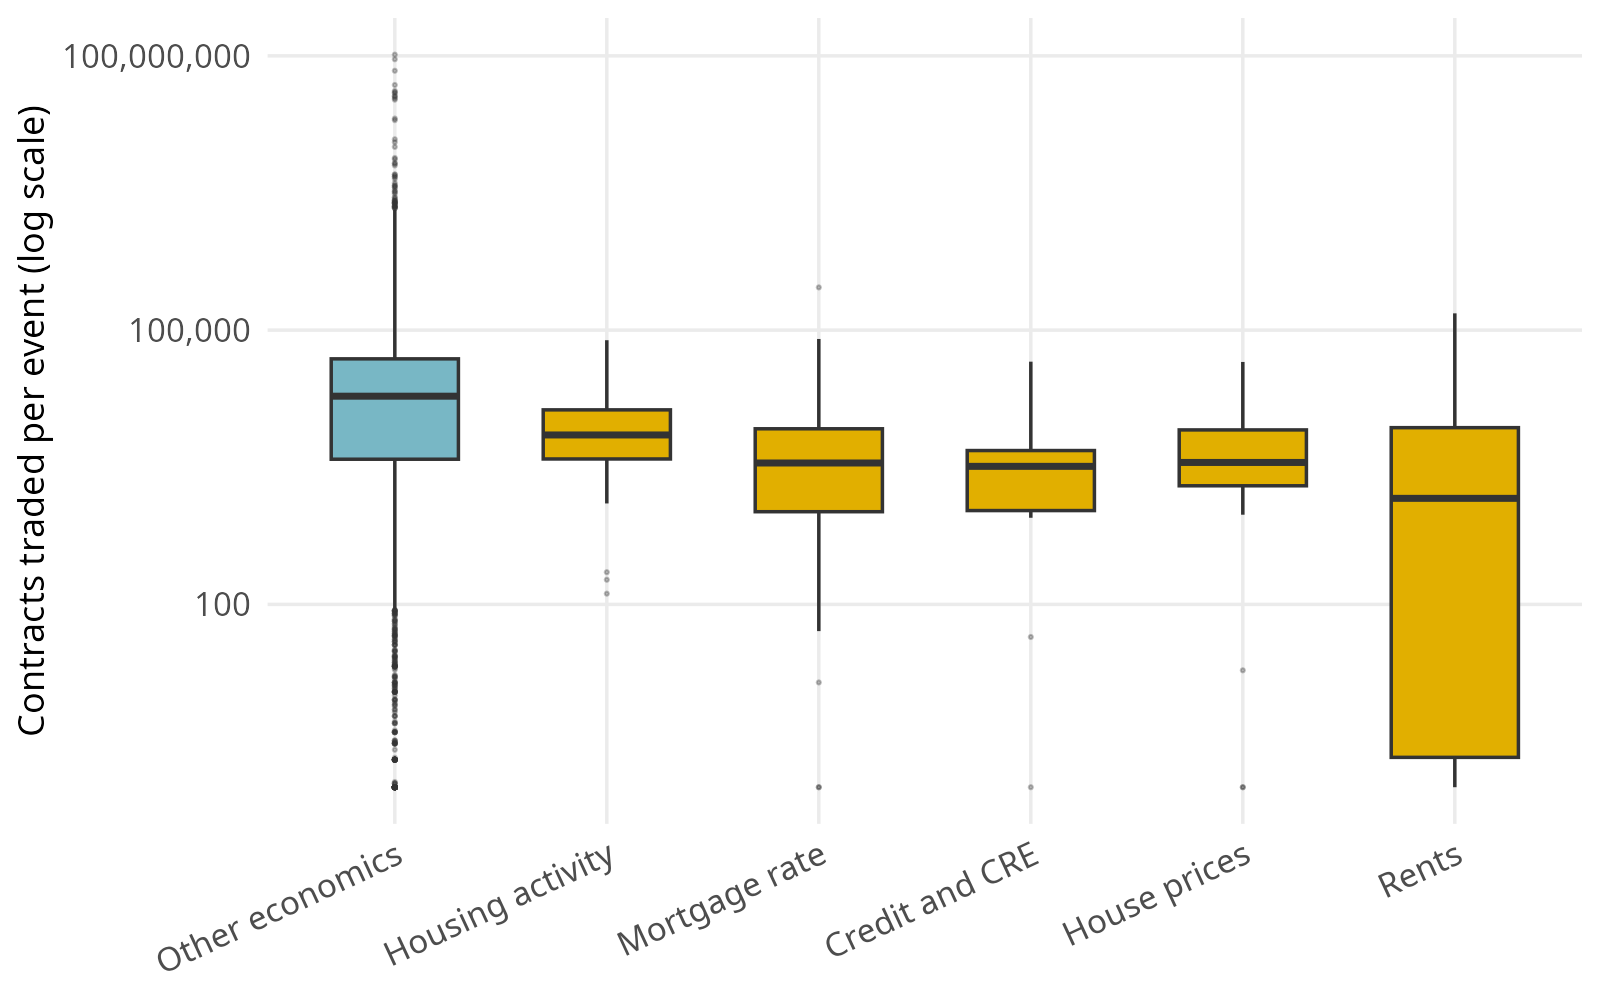
\includegraphics[width=0.85\textwidth]{figures/event_volume_by_group.png}
\par\vspace{0.3em}
\parbox{\textwidth}{\footnotesize\textit{Notes: Closed events. Volume is summed over the strikes of each event and plotted as volume plus one on a log scale.}}
\end{figure}

\subsection{Conditional comparison}

Table~\ref{tab:regression} regresses log event volume on a real estate indicator, with standard errors clustered by series. Unconditionally a real estate event trades \uncondGap{} per cent less than another economics event (column 1), and controlling for the listing horizon, the number of strikes and the quarter of closing narrows the gap only to \condGap{} per cent (column 2).

I expected liquidity to fall away at longer horizons, since that is where the mismatch between speculators and hedgers should bite, but the data do not show it. Volume rises with the listing horizon, as it must when volume is cumulative, and the slope for real estate events is no different (column 3). The more telling fact is that there are no long horizons to observe: the exchange does not list a five-year house price contract of the kind the CME added in 2007 \citep{shiller2008derivatives}, and that is a fact about what gets listed and not an estimate of anything.

Column 4 looks at fragmentation. Among other economics events, volume per strike does not fall as strikes are added, whereas among real estate events it falls with an elasticity of about \strikeElasticity{}. Taken at face value this would mean that extra strikes in real estate divide a fixed pool of interest, in the way the concentration argument of \citet{pagano1989trading} predicts, while elsewhere the exchange adds strikes where there is interest to fill them. Figure~\ref{fig:strikes} plots every event, with the number of strikes it lists on the horizontal axis and the contracts traded per strike on the vertical axis, and adds a fitted line for each group: the line for real estate slopes down more steeply than the line for the other events. I would not lean on it, because only \reEventsManyStrikes{} of the \regReEvents{} real estate events list more than ten strikes, so that the right-hand end of the real estate line rests on few points, and because the exchange chooses the number of strikes with expected demand in mind. Quotes give a mixed picture of the cost of longer ladders. For other economics contracts the median quoted spread lies between \spreadBinMin{} and \spreadBinMax{} cents whatever the number of strikes in the event, whereas for real estate it rises from \spreadReOneStrike{} cents in single-strike events to \spreadReManyStrikes{} cents in events with eleven to fifteen strikes (Table~\ref{tab:spreadstrikes} in the appendix). With the controls of Table~\ref{tab:quotes}, however, more strikes do not go with wider spreads, and the relation is no different for real estate. Depth is taken up in Section~\ref{sec:household}.

\begin{table}[H]
\centering\small
\caption{\textbf{Event volume: real estate against other economics events}}
\label{tab:regression}
\begin{tabular}{lcccc}
\toprule
 & (1) & (2) & (3) & (4) \\
 & log volume & log volume & log volume & log volume per strike \\
\midrule
\tabinput{tables/regression}
\bottomrule
\end{tabular}
\par\vspace{0.4em}
\parbox{\textwidth}{\footnotesize\textit{Notes: OLS on closed events. Volume enters as log(1 + contracts traded). Standard errors clustered by series in parentheses. *** p < 0.01, ** p < 0.05, * p < 0.10.}}
\end{table}

\begin{figure}[H]
\centering
\caption{\textbf{Contracts traded per strike against the number of strikes}}
\label{fig:strikes}
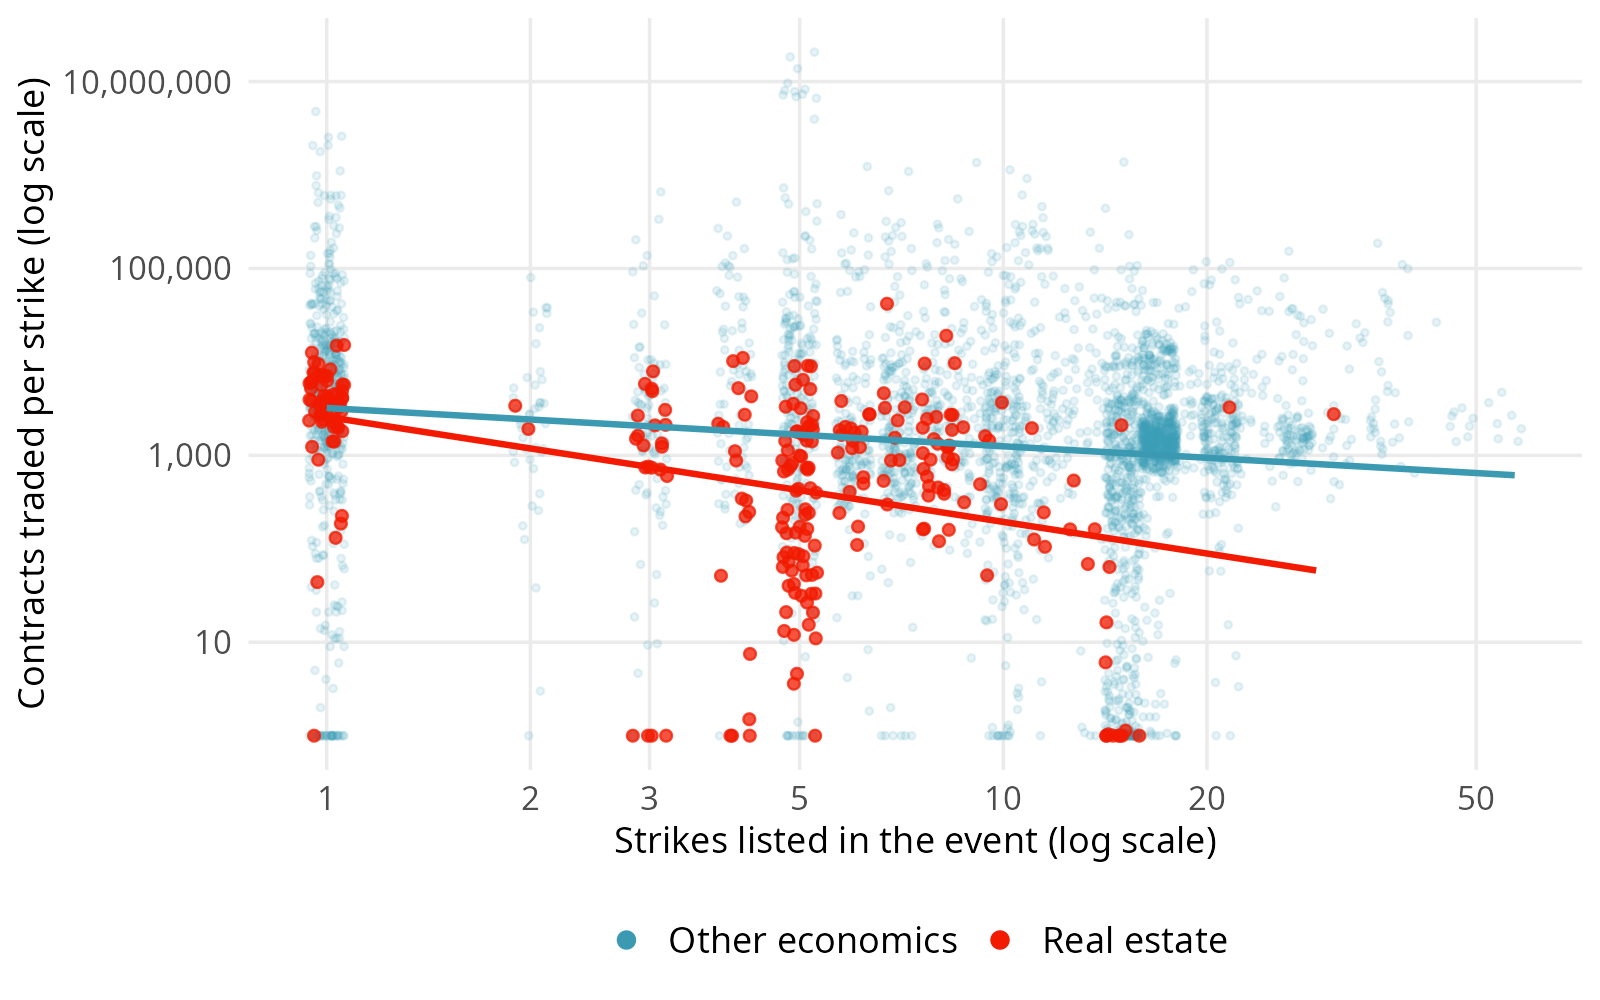
\includegraphics[width=0.85\textwidth]{figures/volume_per_strike_by_strikes.png}
\par\vspace{0.3em}
\parbox{\textwidth}{\footnotesize\textit{Notes: Each point is one closed event. The horizontal axis is the number of strikes (markets) listed in the event, slightly jittered, and the vertical axis is the event's volume divided by that number, plotted as one plus the value so that events without any trade appear at the bottom. Lines are least-squares fits in logs for each group.}}
\end{figure}

\subsection{Quotes and price accuracy}

Volume does not say what it would have cost to trade or whether the prices were any good. Daily candlesticks give closing bid and ask quotes for every real estate market listed for at least two days and for a fixed sample of about a quarter of the other economics markets with the same restriction. After dropping markets that have not settled, \quoteMarkets{} markets remain, \quoteReMarkets{} of them real estate; Table~\ref{tab:quotes_summary} summarises them and Table~\ref{tab:quotesgroup} in the appendix breaks the measures down by group.

Real estate contracts are quoted like any other. The median quoted spread is \spreadComparison{}, and with controls for horizon and quarter the two groups do not differ significantly (Table~\ref{tab:quotes}, column 1). Real estate markets have a two-sided quote on \twoSidedRe{} per cent of days against \twoSidedOther{} per cent elsewhere, a gap of \twoSidedGap{} points with controls (column 2). Somebody posts prices in these markets, which is consistent with the account of \citet{diercks2026kalshi}, who note that Kalshi is supported by professional market makers such as Susquehanna. What is missing is anyone to take the other side: house price markets trade on \priceDaysTraded{} per cent of days and rent markets on \rentDaysTraded{} per cent, against \otherDaysTraded{} per cent for the comparison group (Table~\ref{tab:quotesgroup}). Nor is a spread of \spreadRe{} cents cheap, since on a contract priced at 50 cents it amounts to a round trip of \spreadRoundTrip{} per cent, and the data say nothing about how much could be traded at the quote.

Their prices are also about as accurate. I take as the forecast the quote midpoint one day or seven days before close, or the last trade price when the book is one-sided, and treat it as a probability in the sense of \citet{wolfers2006interpreting}. The raw Brier score is worse for real estate, \brierRe{} against \brierOther{} one day out, but real estate prices sit closer to 50 cents, where any forecast scores worse. Conditional on $p(1-p)$ the difference is \brierDiff{} and insignificant (Table~\ref{tab:quotes}, column 3), and the same holds seven days out (column 4). A regression of outcomes on prices gives a slope of \calSlope{} with no difference for real estate (column 5), and Figure~\ref{fig:calibration} shows both groups close to the diagonal. This matches what \citet{diercks2026kalshi} find for Kalshi's macroeconomic contracts, whose forecasts are about as accurate as the Bloomberg consensus, and what \citet{gurkaynak2006macroeconomic} found for the economic derivatives auctions two decades earlier.

Information about future prices is the first of the four benefits that \citet{fabozzi2020thirty} list for property derivatives, ahead of hedging, portfolio diversification and a basis for new financial products, and it is the only one these contracts deliver. Even that conclusion rests on thin evidence where house prices are concerned, because only \priceForecastN{} house price markets have a one-day forecast and all of them resolve within months of listing.

\begin{table}[H]
\centering\small
\caption{\textbf{Summary statistics, markets with quote data}}
\label{tab:quotes_summary}
\begin{tabular}{lrrrrrr}
\toprule
 & N & Mean & SD & Min & Median & Max \\
\midrule
\tabinput{tables/quotes_summary}
\bottomrule
\end{tabular}
\par\vspace{0.4em}
\parbox{\textwidth}{\footnotesize\textit{Notes: Settled markets listed for at least two days: all real estate markets and a fixed sample of other economics markets, chosen by a hash of the market identifier so that it stays the same across updates. Spreads are in dollars per one-dollar contract and are defined on days with both a bid and an ask. The Brier score is the squared difference between price and outcome. The last row is an indicator for markets in any of the five real estate groups.}}
\end{table}

\begin{table}[H]
\centering\small
\caption{\textbf{Quotes and forecast accuracy: real estate against other economics markets}}
\label{tab:quotes}
\begin{tabular}{lccccc}
\toprule
 & (1) & (2) & (3) & (4) & (5) \\
 & Spread & Two-sided & Brier, 1 day & Brier, 7 days & Outcome \\
\midrule
\tabinput{tables/quotes_regression}
\bottomrule
\end{tabular}
\par\vspace{0.4em}
\parbox{\textwidth}{\footnotesize\textit{Notes: OLS on settled markets. Spread is the market's median quoted spread; two-sided is the share of days with both a bid and an ask. Column 5 regresses the outcome (1 if yes) on the price one day before close. Standard errors clustered by event in parentheses. *** p < 0.01, ** p < 0.05, * p < 0.10.}}
\end{table}

\begin{figure}[H]
\centering
\caption{\textbf{Calibration one day before close}}
\label{fig:calibration}
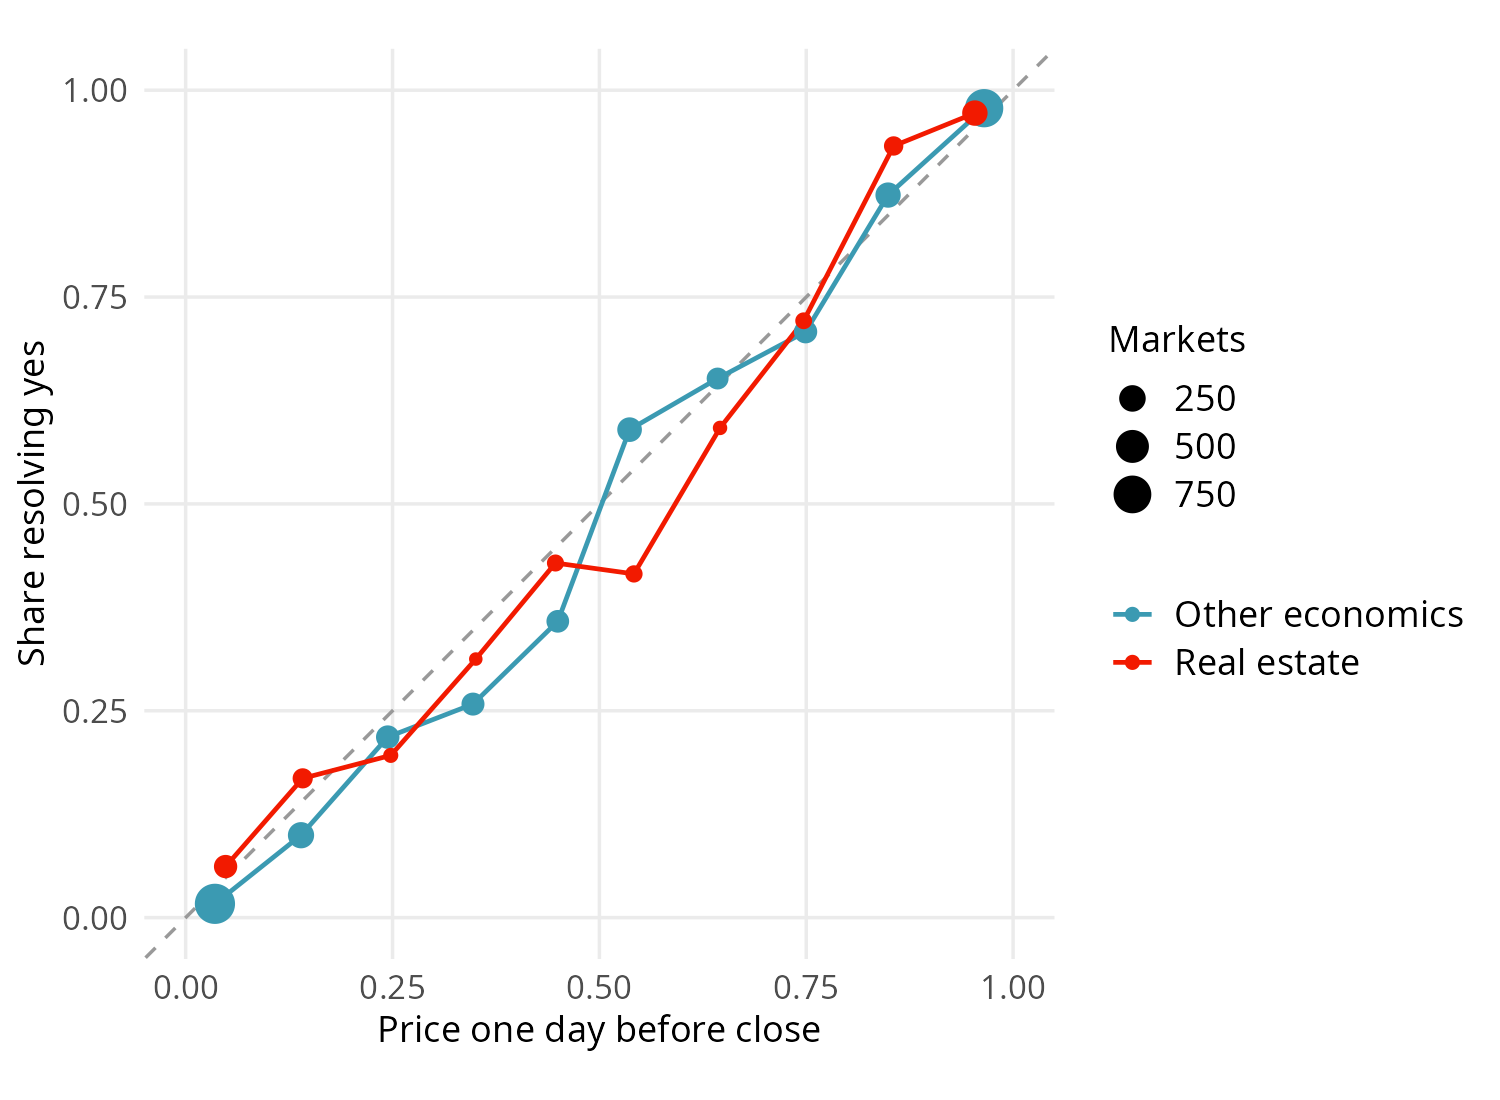
\includegraphics[width=0.75\textwidth]{figures/calibration_one_day.png}
\par\vspace{0.3em}
\parbox{\textwidth}{\footnotesize\textit{Notes: Markets are grouped into ten bins by price one day before close. Each point is the mean price and the share of markets in the bin that resolved yes.}}
\end{figure}

\subsection{Hedging capacity of an index contract}

Suppose the contracts were liquid. To see how much of an owner's price risk they could then remove, I use the Cook County Assessor's parcel sales \citep{cookcounty2026sales}, which are public and cover \cookSalesM{} million residential sales in and around Chicago. After dropping sales before 2000, multi-parcel sales, sales below 10,000 dollars, non-warranty deeds and the assessor's flagged duplicates, and keeping houses and condominiums, consecutive sales of the same parcel at least six months apart give \pairs{} repeat-sale pairs on \pairProperties{} properties, from which the top and bottom one per cent of annualised returns within each holding-period group are trimmed. For each pair, the log price change of the house is regressed on the payoff of a hedge written on the S\&P/Case-Shiller Chicago index \citep{spcaseshiller2026} over the same months, and the $R^2$ of that regression is the share of house-level variance the hedge removes, which is the measure of hedging effectiveness that \citet{bertus2008hedging} apply to Las Vegas. Chicago is one of the ten cities for which the CME listed futures \citep{fabozzi2020thirty} and one of the areas for which Polymarket lists event contracts.

Table~\ref{tab:hedging} and Figure~\ref{fig:hedging} give the result by holding period. For owners who sell within two years a position in the index removes at most \hedgeUnderTwo{} per cent of the variance of their price change, and the share then rises to \hedgeTwoThree{} per cent at two to three years, \hedgeThreeFive{} per cent at three to five and \hedgeFiveTen{} per cent at five to ten. This is the pattern that \citet{giacoletti2021idiosyncratic} documents for California and \citet{eichholtz2021total} for Amsterdam, and it is the opposite of what the exchanges supply: the longest real estate contract on Kalshi ran \reMaxHorizon{} days and the longest house price contract on Polymarket \polyMaxHorizon{} days, and at those horizons there is almost nothing for an index contract to hedge.

The payoff shape matters much less than the horizon. A ladder of seven binary contracts, with strikes at evenly spaced quantiles of the index change, removes as much variance as a linear position at every holding period (Table~\ref{tab:hedging}), as the spanning argument of \citet{ross1976options} implies it should. Seven is the median number of strikes per house price event on Kalshi, and Polymarket lists about as many. A single binary on whether the index rose does nearly as well up to five years (\binaryThreeFive{} per cent against \hedgeThreeFive{} at three to five) and much worse beyond ten (\binaryTenPlus{} against \hedgeTenPlus{}). Binary payoffs are therefore not what makes these contracts poor hedges, provided there is a ladder and somebody fills it.

The headline shares come from one episode, however. When the pairs are split by purchase date (Table~\ref{tab:hedgingperiod} in the appendix), the index removes \earlyThreeFive{} per cent of variance at three to five years and \earlyFiveTen{} per cent at five to ten for houses bought in 2000--2011, whose holding periods span the boom and the bust, but only \lateThreeFive{} and \lateFiveTen{} per cent for houses bought from 2012 on. The idiosyncratic component did not grow between the two periods; the index simply moved less, with a standard deviation of its change at five to ten years of \sdIndexLate{} against \sdIndexEarly{} in the earlier group. New York gives the same answer for a calm period: the city's public sales file \citep{nyc2026sales} starts in 2016, and for one- to three-family houses and condominium units there the Case-Shiller New York index removes at most \nycMaxR{} per cent of house-level variance at any holding period up to ten years (Table~\ref{tab:hedgingrobust}). An index hedge, in other words, protects against a market-wide crash of the kind that \citet{fabozzi2020thirty} have in mind, and in ordinary years it does almost nothing for the owner of one house.

These numbers are upper bounds, because the hedge is assumed to match the holding period exactly, hedge ratios are fitted in sample (and \citet{bertus2008hedging} caution that they change over time), and the index is taken as final, which ignores the revisions documented by \citet{clapham2006revisiting}. They also concern price risk only. An owner who lets the property earns a total return that includes the rental yield, and since \citet{eichholtz2021total} show that the yield accounts for an increasing part of property-level risk at longer horizons, the hedgeable share of total return risk is lower than the shares reported here for prices. Short holding periods are moreover a selected sample, heavy with renovated resales and distressed sales, which is one reason the fitted hedge ratio is negative below one year, so the two-year result should be read as ``no evidence of hedgeable risk'' and not as a precise zero. Including all deed types in Cook County in place of warranty deeds only leaves the pattern unchanged (Table~\ref{tab:hedgingrobust}). The New York file has no flag for arm's-length sales and the Case-Shiller New York index covers the whole metropolitan area, so that comparison is rougher than the one for Chicago.

\begin{table}[H]
\centering\small
\caption{\textbf{Share of house-level price variance removed by a Case-Shiller Chicago hedge}}
\label{tab:hedging}
\begin{tabular}{lrrrrrrr}
\toprule
 & & \multicolumn{2}{c}{SD of log change} & & \multicolumn{3}{c}{$R^2$ of hedge} \\
\cmidrule(lr){3-4}\cmidrule(lr){6-8}
Holding (years) & Pairs & House & Index & Hedge ratio & Linear & Seven binaries & One binary \\
\midrule
\tabinput{tables/hedging}
\bottomrule
\end{tabular}
\par\vspace{0.4em}
\parbox{\textwidth}{\footnotesize\textit{Notes: Repeat-sale pairs of houses and condominiums in Cook County, Illinois, sold from 2000 on, warranty deeds. Each row regresses the log price change of the house on the hedge payoff over the same months. Linear is the log change of the S\&P/Case-Shiller Chicago index; the hedge ratio is its slope. One binary pays if the index rose. Seven binaries have strikes at evenly spaced quantiles of the index change within the row.}}
\end{table}

\begin{figure}[H]
\centering
\caption{\textbf{Hedgeable share of house price variance by holding period}}
\label{fig:hedging}
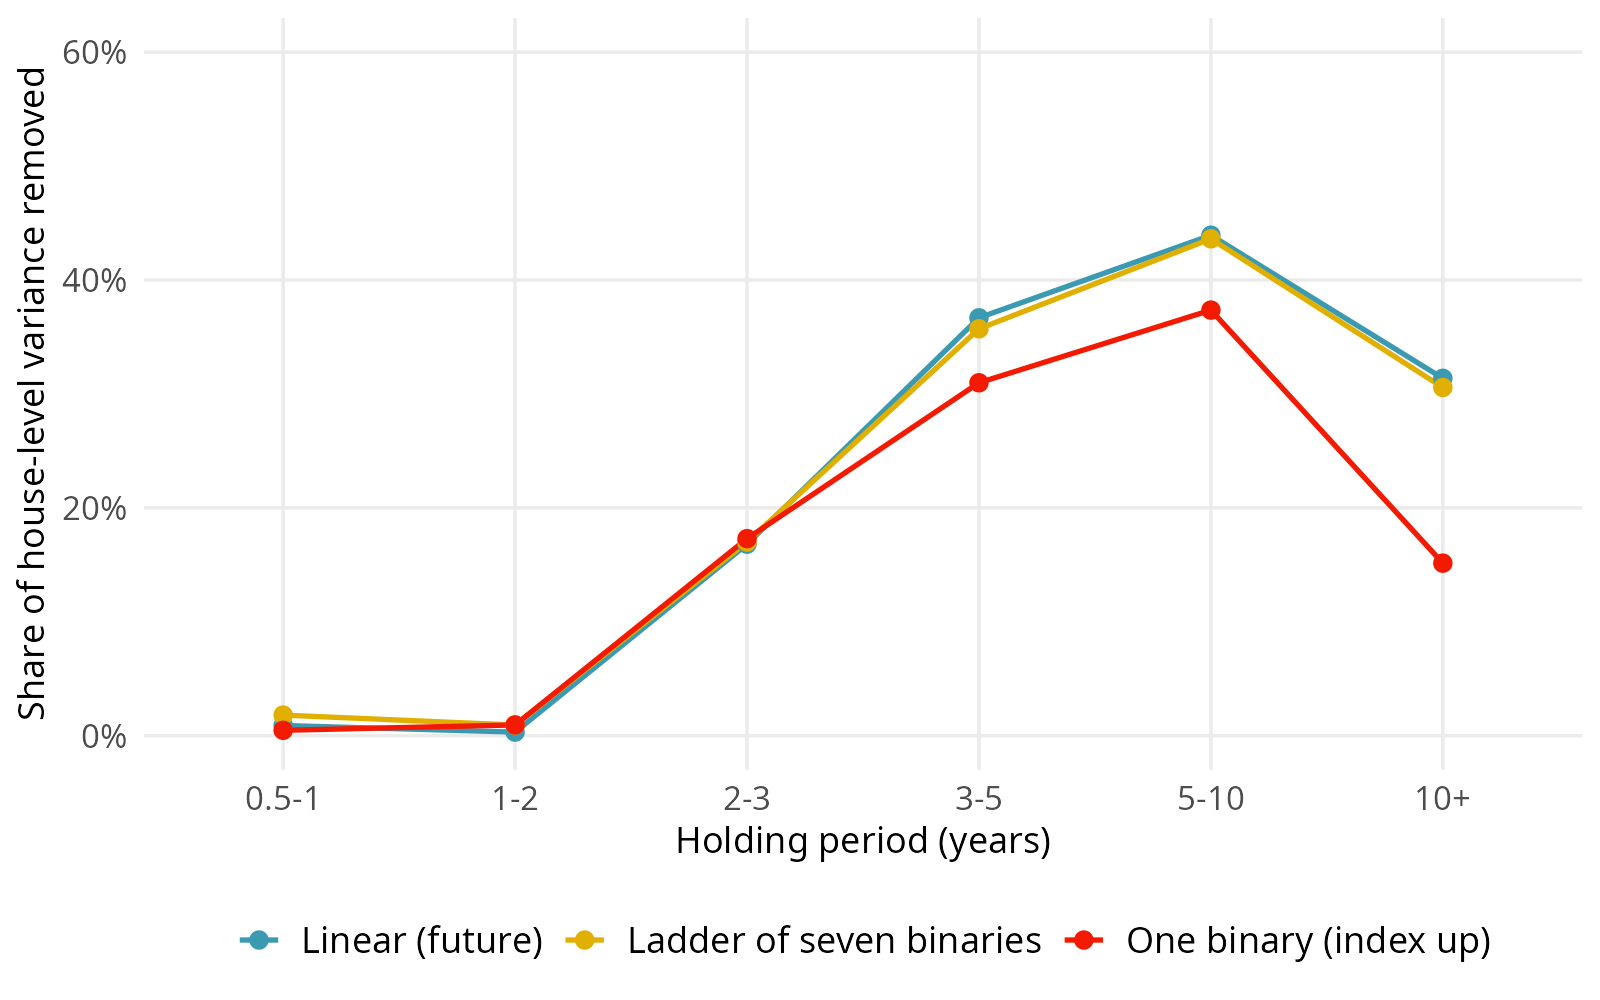
\includegraphics[width=0.85\textwidth]{figures/hedging_by_holding_period.png}
\par\vspace{0.3em}
\parbox{\textwidth}{\footnotesize\textit{Notes: $R^2$ from Table~\ref{tab:hedging}.}}
\end{figure}

\subsection{A second exchange}

Polymarket has listed house price contracts since \polyLaunch{}. Each event asks what the median home value in a metropolitan area will be on a given date and offers \polyBracketsMin{} to \polyBracketsMax{} price brackets, and by \dataMonth{} the contracts covered the United States and \polyMetros{} metropolitan areas. According to the contract rules published with each event, they settle on the Parcl Labs sales price index for the area, a price per square foot published daily, multiplied by a fixed median home size. I found the events by keyword search, since the exchange has no housing category, and dropped contracts on political acts such as housing bills.

The \polyEvents{} house price events traded \polyPriceVolM{} million contracts up to \dataMonth{}. The exchange's volume figure counts contracts, each paying one dollar if its bracket is hit, and it matches the number of contracts in the trade records; the dollars that takers actually paid for them come to \polyTakerUsdM{} million. Either way this is more than Kalshi's house price contracts have traded since \firstOpen{} and still a rounding error against the CME figure. Table~\ref{tab:cohorts} follows the volume by launch month. The first monthly events, opened in January 2026, traded a median of \polyJanMedian{} contracts each, and for the events opened from March to June the median had fallen to \polyMarJunMedian{}. In July the exchange replaced the monthly contracts with quarterly ones, which traded a median of \polyJulyMedian{} contracts per event; the longest contract runs \polyMaxHorizon{} days. I cannot say how much of the July jump is organic. The exchange pays liquidity rewards on the contracts that are open at the time of writing, according to its own market data, but it does not report whether the contracts that have since closed carried them, and several of the largest wallets collect such rewards across the exchange (Table~\ref{tab:topwallets}).

Polymarket settles on a public blockchain, so each trade carries the wallet addresses of both sides. A wallet is an account and not a person, and one person can hold several, but the addresses do show what kind of participation there is. The house price markets saw \polyTx{} transactions among \polyWallets{} wallets, with takers paying \polyTakerUsd{} dollars. The median wallet traded \walletMedianUsd{} dollars in total, counting both sides; \walletUnderHundred{} per cent of wallets traded less than 100 dollars and only \bigWallets{} traded more than 10,000. The ten largest account for \topTenWalletShare{} per cent of the dollars, and \walletOneMonth{} per cent of wallets appear in the contracts of a single launch month and never again, the number of active wallets by launch month being shown in Table~\ref{tab:cohorts}.

Table~\ref{tab:wallets} sorts wallets by two measures: the share of their dollars that came from resting orders filled by someone else, and the ratio of their net position to their gross trading, market by market. A wallet with most of its dollars in resting orders and little net position is providing liquidity, whereas one that takes prices and keeps what it buys holds a view. By that sorting, \mmWallets{} wallets with \mmShare{} per cent of the dollars provide liquidity and \holdWallets{} wallets with \holdShare{} per cent take a position and hold it. Among the \bigWallets{} wallets above 10,000 dollars, \bigHold{} take and hold, \bigRound{} take and trade out again, and \bigMM{} provide liquidity; Table~\ref{tab:topwallets} in the appendix profiles the largest individually.

The large wallets are generalists (Table~\ref{tab:topwallets}). The median one among the \bigWallets{} has traded about \bigMedianMarkets{} markets across the exchange, \bigRewarded{} have collected more than 1,000 dollars in the exchange's liquidity rewards, and \bigRewardedLarge{} more than 100,000, so that for them a house price contract is one more market to quote or one more bet. Of the \topProfiled{} largest wallets, \housingOnly{} have traded house price markets and nothing else. Who they are cannot be told from an address. A wallet that only ever trades one sponsor's contracts could belong to the index provider or to the exchange, in which case part of the recorded volume would be seeding and not demand, but that is conjecture. The largest wallet of all, with \topWalletShare{} per cent of the dollars, bought in a single launch month, held, and did not come back.

What the records show, then, is a crowd trying a new product for the price of a coffee, a few larger accounts placing bets, and professional liquidity providers who quote these contracts because they quote everything. No account looks like a household covering a six-figure exposure, and none is big enough to be an institution doing so, the largest having traded \topWalletUsd{} dollars. These are not the pension funds, insurers and hedge funds that \citet{fabozzi2020thirty} expected to carry the other side of a property derivatives market. Kalshi publishes trades without identities, so the same count cannot be made there, although \citet{diercks2026kalshi} describe its users as a mix of market-making firms and retail traders reached through brokerage apps.

\begin{table}[H]
\centering\small
\caption{\textbf{Wallets in Polymarket house price markets, by trading behaviour}}
\label{tab:wallets}
\begin{tabular}{lrrrr}
\toprule
 & Wallets & Dollars (\%) & Median dollars & Above \$10,000 \\
\midrule
\tabinput{tables/wallet_types}
\bottomrule
\end{tabular}
\par\vspace{0.4em}
\parbox{\textwidth}{\footnotesize\textit{Notes: All trades in Polymarket contracts on median home values, \polyLaunch{} to \dataMonth{}. Dollars are summed over both sides of each trade. A wallet rests orders if at least half its dollars came from orders filled by another party. It ends flat, or trades out, if the absolute net position summed over markets is less than half its gross trading, in shares.}}
\end{table}

\begin{table}[H]
\centering\small
\caption{\textbf{Polymarket house price events by launch month}}
\label{tab:cohorts}
\begin{tabular}{lrrrrrr}
\toprule
Launched & Events & Contracts (000) & Median & Paid (\$000) & Days & Wallets \\
\midrule
\tabinput{tables/polymarket_cohorts}
\bottomrule
\end{tabular}
\par\vspace{0.4em}
\parbox{\textwidth}{\footnotesize\textit{Notes: Events grouped by the month they opened. Contracts is volume as reported by the exchange and median is the median across events. Paid is what takers paid for those contracts according to the trade records, days is the median listing horizon, and wallets is the number of distinct addresses on either side of a trade. The latest cohorts are still open.}}
\end{table}

\subsection{A household's hedge}\label{sec:household}

There is little sign that homeowners try to hedge, and the markets could not take such a hedge if one did. The earlier record already points that way. \citet{caplin2003home} review the home equity assurance programmes run by Illinois municipalities, which insured owners against local price declines at a heavily subsidised price, and report that only 15 per cent of owner-occupiers in Oak Park took the insurance and that take-up elsewhere was generally below 10 per cent. \citet{shiller2008derivatives} puts the open interest in the Goldman Sachs house price warrants of 2004 at what would hedge about a hundred houses. Polymarket's trade records allow a direct look. A household hedging its home would trade the contracts for one area, come back each time they are relisted, keep what it buys, and stay on one side of the market's consensus, below it for an owner and above it for a renter who wants to buy. Of the \hedgerCandidates{} wallets that traded at least 1,000 dollars in two or more launch months, \hedgerOneArea{} concentrate four fifths of their trading on one area, of which \hedgerLike{} also kept a one-sided position, the largest of these having traded about \hedgerLikeUsd{} dollars in all. That is too small to cover anything, and it may just as well be a local with an opinion.

Nor could the markets absorb a real hedge. An owner of a 500,000 dollar home who wants cover against a 10 per cent fall needs contracts that pay 50,000 dollars. Table~\ref{tab:depth} summarises the order books of all open house price contracts on \depthDate{}. Adding up, across the strikes of an event, the contracts on offer within five cents of the best quote gives a median of \depthKalshiMedian{} dollars of payout per event on Kalshi and \depthPolyMedian{} on Polymarket, taking the deeper side of each book, which is \depthMedianShare{} per cent of what this one household needs. The deepest event on either exchange offers \depthMaxShare{} per cent. The largest net position any wallet has ever held in a Polymarket house price event is about \maxNetPosition{} contracts. Prices would move long before that. Walking through each book from the best quote, an order for 100 contracts fills within five cents on \fillNearHundred{} per cent of book sides, but an order for 1,000 contracts does so on only \fillNearThousand{} per cent and, where the book can fill it at all, moves the price by a median of \moveThousand{} cents on a contract that pays a dollar (Table~\ref{tab:impact} in the appendix). Spreading the hedge over a ladder of seven strikes still means buying about 7,000 contracts in each, which \fillLadder{} per cent of book sides could fill at any price and \fillNearLadder{} per cent within five cents, and no book holds the 50,000 contracts that a single-strike hedge would take. A single homeowner would therefore exhaust the quotes of a metropolitan market, moving prices by tens of cents on the way, and would have to do so again every few months as contracts expire. The snapshot is one moment, and market makers may refill their quotes after a trade, but there is no sign of standing capacity on the scale of even a handful of houses.

\begin{table}[H]
\centering\small
\caption{\textbf{Order book depth of open house price contracts}}
\label{tab:depth}
\begin{tabular}{lrrrrrrr}
\toprule
 & & & \multicolumn{3}{c}{On offer per event (dollars)} & \multicolumn{2}{c}{Whole book} \\
\cmidrule(lr){4-6}\cmidrule(lr){7-8}
 & Events & Markets & At best & Near, median & Near, max & Median & Max \\
\midrule
\tabinput{tables/depth}
\bottomrule
\end{tabular}
\par\vspace{0.4em}
\parbox{\textwidth}{\footnotesize\textit{Notes: Order books of open contracts on house prices, recorded on \depthDate{}. Each contract pays one dollar, so the number of contracts on offer is the payout a trader could buy. Contracts are summed over the strikes of an event, separately for buyers of yes and buyers of no, and the deeper side is reported. At best is the median across events of the payout on offer at the best quote; near counts offers within five cents of it. The whole book includes offers far from the best quote.}}
\end{table}

\subsection{Other real estate contracts on Polymarket}

The two exchanges use different index providers and different contract designs and end up at the same order of magnitude. Polymarket's other real estate contracts are few: \polyMortgageEvents{} events on the 30-year mortgage rate since 2022 and \polyOtherEvents{} others, one on a mortgage delinquency rate and one on the level of the Dubai Financial Market's real estate share index, which tracks listed companies and not property prices.

\section{Open work}

The hedging test uses Case-Shiller, which is not what the event contracts settle on, and it should be rerun against Zillow's and Parcl's indices, for a second city with a long sales history, and out of sample, with hedge ratios set before the holding period begins, since \citet{bertus2008hedging} show that such ratios drift.

The record of the CME housing futures after 2007 is taken here from \citet{fabozzi2020thirty}, without volume and open interest figures of my own. Depth is known for a single day only. Neither exchange archives its order book, so the pipeline now records a snapshot at every update, and a history of depth will build up from here.

Polymarket is covered through event volume and trades by wallet, but its quotes and price accuracy have not been analysed, and the identity of the wallets that trade only housing contracts remains open.

\bibliographystyle{plainnat}
\bibliography{references}

\appendix
\section{Supporting tables}

\begin{footnotesize}
\begin{longtable}{lp{4.3cm}rrrll}
\caption{\textbf{Real estate series on Kalshi}}\label{tab:series}\\
\toprule
Series & Title & Events & Markets & Contracts (000) & First & Last \\
\midrule
\endfirsthead
\toprule
Series & Title & Events & Markets & Contracts (000) & First & Last \\
\midrule
\endhead
\tabinput{tables/re_series}
\bottomrule
\end{longtable}
\end{footnotesize}
\noindent{\footnotesize\textit{Notes: All series classified as real estate, sorted by volume within group. Titles as given by the exchange, truncated. Last close can lie in the future for open markets.}}

\begin{table}[H]
\centering\small
\caption{\textbf{Quotes and forecast accuracy by group}}
\label{tab:quotesgroup}
\begin{tabular}{lrrrrrrrr}
\toprule
 & & \multicolumn{2}{c}{Share of days (\%)} & & \multicolumn{2}{c}{One day} & \multicolumn{2}{c}{Seven days} \\
\cmidrule(lr){3-4}\cmidrule(lr){6-7}\cmidrule(lr){8-9}
 & Markets & Two-sided & Traded & Spread (cents) & N & Brier & N & Brier \\
\midrule
\tabinput{tables/quotes_by_group}
\bottomrule
\end{tabular}
\par\vspace{0.4em}
\parbox{\textwidth}{\footnotesize\textit{Notes: Settled markets with quote data. Shares of days are means across markets, the spread is the median across markets of each market's median quoted spread, and N is the number of markets with a forecast at that lead.}}
\end{table}

\begin{table}[H]
\centering\small
\caption{\textbf{Median quoted spread by number of strikes in the event}}
\label{tab:spreadstrikes}
\begin{tabular}{lrrrr}
\toprule
 & \multicolumn{2}{c}{Other economics} & \multicolumn{2}{c}{Real estate} \\
\cmidrule(lr){2-3}\cmidrule(lr){4-5}
Strikes & Markets & Spread (cents) & Markets & Spread (cents) \\
\midrule
\tabinput{tables/spread_by_strikes}
\bottomrule
\end{tabular}
\par\vspace{0.4em}
\parbox{\textwidth}{\footnotesize\textit{Notes: Settled markets with quote data, grouped by the number of markets listed in the same event. The spread is the median across markets of each market's median quoted spread.}}
\end{table}

\begin{table}[H]
\centering\small
\caption{\textbf{Price impact of orders in open house price contracts}}
\label{tab:impact}
\begin{tabular}{rrrrrrr}
\toprule
 & \multicolumn{3}{c}{Kalshi} & \multicolumn{3}{c}{Polymarket} \\
\cmidrule(lr){2-4}\cmidrule(lr){5-7}
Order & Fillable (\%) & Near (\%) & Move (cents) & Fillable (\%) & Near (\%) & Move (cents) \\
\midrule
\tabinput{tables/price_impact}
\bottomrule
\end{tabular}
\par\vspace{0.4em}
\parbox{\textwidth}{\footnotesize\textit{Notes: Order books of open house price contracts on \depthDate{}, one observation per market and side. Order is the number of contracts bought. Fillable is the share of book sides holding at least that number at any price, and near the share that can fill the order without the price moving more than five cents from the best quote. Move is the median distance in cents from the best quote to the price of the last contract filled, among book sides that can fill the order. A hedge of 50,000 dollars takes 50,000 contracts at one strike or about 7,000 at each of seven.}}
\end{table}

\begin{table}[H]
\centering\small
\caption{\textbf{Linear index hedge by purchase period, Cook County}}
\label{tab:hedgingperiod}
\begin{tabular}{lrrrr}
\toprule
Holding (years) & Pairs & SD of index change & Hedge ratio & $R^2$ \\
\midrule
\tabinput{tables/hedging_by_period}
\bottomrule
\end{tabular}
\par\vspace{0.4em}
\parbox{\textwidth}{\footnotesize\textit{Notes: The linear hedge of Table~\ref{tab:hedging}, estimated separately by the date of the first sale in each pair.}}
\end{table}

\begin{table}[H]
\centering\small
\caption{\textbf{Linear index hedge in alternative samples}}
\label{tab:hedgingrobust}
\begin{tabular}{lrrrrrr}
\toprule
 & \multicolumn{2}{c}{Cook County, warranty deeds} & \multicolumn{2}{c}{Cook County, all deeds} & \multicolumn{2}{c}{New York City} \\
\cmidrule(lr){2-3}\cmidrule(lr){4-5}\cmidrule(lr){6-7}
Holding (years) & Pairs & $R^2$ & Pairs & $R^2$ & Pairs & $R^2$ \\
\midrule
\tabinput{tables/hedging_robust}
\bottomrule
\end{tabular}
\par\vspace{0.4em}
\parbox{\textwidth}{\footnotesize\textit{Notes: $R^2$ of the house's log price change on the log change of the S\&P/Case-Shiller index for the city. The New York sales file starts in 2016, so no pair is held for ten years.}}
\end{table}

\begin{table}[H]
\centering\footnotesize
\caption{\textbf{The largest wallets in Polymarket house price markets}}
\label{tab:topwallets}
\begin{tabular}{rrrrrrrrlrr}
\toprule
 & & Share & & & Launch & Maker & Net / & & Markets, & Rewards, \\
Rank & Dollars & (\%) & Trades & Markets & months & (\%) & gross & Behaviour & all & dollars \\
\midrule
\tabinput{tables/top_wallets}
\bottomrule
\end{tabular}
\par\vspace{0.4em}
\parbox{\textwidth}{\footnotesize\textit{Notes: Wallets ranked by dollars traded in house price markets, both sides. Maker is the share of those dollars from resting orders. Net / gross is the absolute net position over gross trading, summed across markets. The last two columns cover the wallet's activity on the whole exchange: markets ever traded and liquidity rewards received, the latter from at most the 500 most recent payments. Addresses are not reported.}}
\end{table}


\end{document}
